%!TEX root = ../Thesis.tex
\section{Multichannel-System in der Cloud (An-Nam Pham)}
Das Unternehmen Stylez betreibt ein Multichannel-Retailing (Mehrgleisiger Vertrieb des Handels). Wie in der Grafik \ref{img:Cloud_Implementierung} auf Seite \pageref{img:Cloud_Implementierung} zu sehen, kann der Kunde sowohl in der Filiale, als auch online per Webshop einkaufen. Gekaufte Waren können bei Bedarf ebenfalls sowohl in einer Filiale als auch online umgetauscht oder zurückgegeben werden (beim Online-Weg: Rücksendung per Post).

Die Aufgabe diese Prozesse zu steuern und zu überwachen, ist ohne Unterstützung von passender IT-Systeme kaum zu bewältigen.\\
Die Lösung für die große Multichannel-Herausforderung lautet Multichannel-System.\\
\\
Das Multichannel-System ist ein Verbund von mehreren Systemen, die dem Unternehmen dabei unterstützen, sämtliche Geschäftsprozesse und das Kundenmangement zu steuern.\\
\\
Im Kapitel \ref{sec:IT-Infrastruktur} wurden die Vorteile für einen Umzug in die Cloud erläutert.
Deswegen soll das Multichannel-System in der Cloud betrieben werden.
Die zentrale Datenbank ist die Datenbasis für das Multichannel-System. Da hier nicht nur Unternehmensdaten, sondern auch vertrauliche Kundendaten gespeichert werden, soll diese Datenbank nicht in die Cloud ausgelagert werden, sondern weiterhin vom Unternehmen betrieben werden.

Dies macht das Ganze zu einer hybriden Cloud, die aus der Private Cloud (zentrale Datenbank) und der Public Cloud besteht.\\
\\
Die folgende Abbildung zeigt die empfohlene Implementierung des Multichannel-Systems in der Hybrid Cloud:
\begin{figure}[H]
\centering
\begin{minipage}[t]{0.8\textwidth}
\fbox{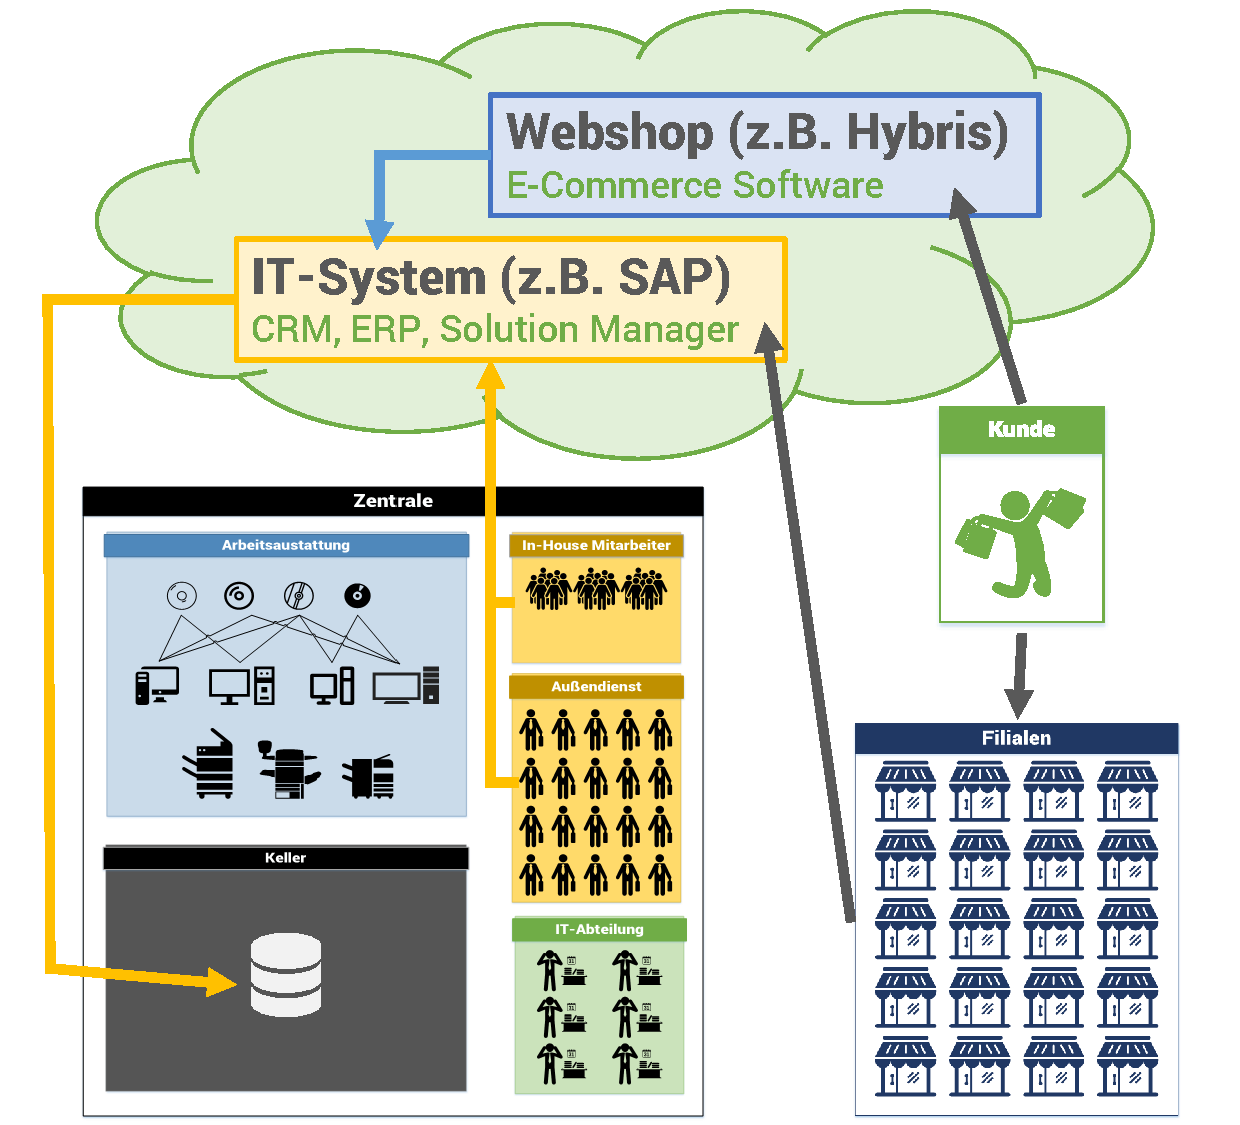
\includegraphics[width=1\textwidth]{img/Cloudinhalt.pdf}}
\caption{Empfohlene Implementierung der Hybrid Cloud} % Überschrift
\source{Eigene Darstellung} % Quelle
\label{img:Cloud_Implementierung}
\end{minipage}
\end{figure}
In den folgenden Unterkapiteln werden die einzelnen Komponenten des Multichannel-Systems kurz beschrieben und ihr Nutzen für das Unternehmen erläutert.
\subsection{SAP IT-System}
Wir empfehlen die gesamte Unternehmensstruktur von Stylez mit Hilfe von SAP im IT-System abzubilden\footnote{Berechtigungskonzept, Organisationsmanagement, Geschäftsprozesse, etc. werden in SAP ERP abgebildet, um ein optimales Business-IT-Alignment zu ermöglichen.}. Der Entscheidung für SAP bietet unter anderem folgende Vorteile\footcite{SAP_Vorteil}:
\begin{itemize}
\item Internationaler Anbieter
\item führende Technologie
\item 40 Jahre Erfahrung mit kfm. Software
\item technische Innovationskraft
\item finanzielle Stabilität
\end{itemize}
Außerdem gibt es viele SAP-Partner, die auf den Fashion-Handel spezialisiert sind. Diese haben unter anderem folgende Stärken:
\begin{itemize}
\item Kundennähe
\item Mittelstandsausrichtung und -erfahrung
\item Angebot als Generalunternehmer
\end{itemize}
Das SAP System soll aus ein \acrshort{ERP}-System, \acrshort{CRM}-System und einen Solution Manager bestehen.
\subsubsection{SAP ERP}
Das \acrlong{ERP}-System (ERP-System) bildet (im Idealfall) das Unternehmen in seiner Gesamtheit zeitnah ab. Dadurch ist es ein sehr wertvolles Hilfsmittel für Planungs- und Steuerungsaufgaben, das unter anderem noch folgende Vorteile bietet:
\begin{itemize}
\item Erhöhte Automatisierung für kürzere Bearbeitungszeiten und Kostenersparnisse
\item Verringerte Durchlaufzeiten von Prozessen
\item Erhöhte Datenqualität, Redundanzen und Inkonsistenzen werden vermieden
\item Verbesserte Zusammenarbeit über Abteilungsgrenzen hinweg
\item Optimierter Informationsfluss im Unternehmen
\item Überwinden organisatorischer und technischer Schnittstellen
\end{itemize}
\underline{\textbf{Der große Nutzen:}}\\
ERP-Systeme tragen langfristig zur Leistungssteigerung und Kostenreduzierung bei, da das ERP-System sämtliche Bereiche wie z.B. Materialwirtschaft, Finanz- und Rechnungswesen, Personalwirtschaft, Verkauf, Marketing und Forschung abbildet. Dadurch können alle Bereiche miteinander kommunizieren und dieselbe Datenbasis nutzen. Dies spart z.B. im Vergleich zur \glqq Zettelwirtschaft\grqq~und Excel viel Zeit und Kosten.\footcite[vgl.][]{ERP}
\subsubsection{SAP CRM}
\glqq Der Kunde ist König\grqq. Dieser bekannte Satz drückt ganz gut aus, worauf man in einem Unternehmen ganz besonders achten muss.\\
Das \acrlong{CRM} (CRM) (zu Deutsch: Kundenbeziehungsmanagement) unterstützt das Unternehmen dabei, die Beziehung zu bestehenden und potenziellen Kunden zu verwalten und zu gestalten.\\
\\
\underline{\textbf{Der große Nutzen:}}\\
Das CRM-System verwaltet nicht nur bestehende und potenzielle Kunden des Unternehmens. Wird das Supply-Chain-Management eingebunden, kann das CRM-System auch Lieferanten verwalten. Im Fall von Stylez können auch alle Franchisenehmer eingebunden werden.\\
Das Besondere am CRM-System ist, dass es die Historie der Kundeninteraktion verfolgbar macht. Es kann sehr schnell ein Überblick über einen Kunden, Lieferanten oder Franchisenehmer\footnote{Zur Vereinfachung werden Kunden, Lieferanten oder Franchisenehmer im Folgenden mit Kunde zusammengefasst.} geschaffen werden (z.B. getätigte Anrufe, Häufigkeit der Support-Anfragen, Anteil am Geschäftsumsatz, uvm.).
Dadurch kann schnell auf den Kunden eingegangen. Dies spart Zeit und fördert die Professionalität und somit auch das Vertrauen der Kunden. Außerdem kann das CRM-Systen benutzt werden, um Prognosen über zu erwartende Ergebnisse einfacher und genauer zu erstellen. Und es bietet volle Transparenz und bei Bedarf jederzeit Zugriff auf Kundeninformationen.\footcite[vgl.][]{CRM}

\subsubsection{SAP Solution Manager}
Der Solution Manager wird für SAP-Kunden kostenfrei mitgeliefert und vereinfacht die Implementierung, den Betrieb, die Überwachung und die Unterstützung von SAP-Produkte im Unternehmen. Dabei bildet der Solution Manager alle IT-Prozesse ab und erfüllt bei der Betreibung dieser Prozesse alle ITIL-Prozesse\footcite[vgl.][]{SAPITIL}.

Folgende Komponenten umfasst der Solution Manager:
\begin{itemize}
\item Implementierung und Upgrade
\item Change Control Management
\item Testunterstützung
\item IT- und Anwendungs-Support
\item Diagnose und Ursachenanalyse
\item Systemüberwachung mit Solution Monitoring
\item Service-Level-Management und Reporting
\item Service-Verarbeitung
\item Administration
\end{itemize}
\underline{\textbf{Der große Nutzen:}}\\
Mit Hilfe des Solution Managers kann die IT-Abteilung der Firma stark entlastet werden. Sämtliche IT-Prozesse wie z.B. der IT- und Answendungs-Support per Helpdesk oder auch die Systemüberwachung und Administration werden vom Solution Manager nach ITIL unterstützt. Dank Solution Manager wird viel Aufwand und Zeit für IT-Aufgaben im Unternehmen eingespart.\footcite[vgl.][]{SolutionManager}

\subsection{Hybris (Webshop)}
Hybris ist ein E-Commerce-, Marketing- und Billing-Produkt\footnote{Abrechnungs-Produkt}, das seit 2013 zu SAP gehört\footcite[vgl.][]{SAPHybris}. Hybris wird für das Unternehmen Stylez empfohlen, da es:
\begin{enumerate}
\item auf Multichannel spezialisiert ist,
\item voll kompatibel mit SAP-Systemen ist und
\item Kundendaten in Echtzeit auswerten kann.
\end{enumerate}
\section{So funktioniert der Umzug in die Hybrid Cloud (An-Nam Pham)}
% \section{Stichwort: Hochverfügbarkeit}
%\section SAP Rapid Deployment Solution
\section{Roadmap (An-Nam Pham)}
